%%%%%%%%%%%%%%%%%%%%%%%%%%%%%%%%%%%%%%%%%
% Beamer Presentation
% LaTeX Template
% Version 1.0 (10/11/12)
%
% This template has been downloaded from:
% http://www.LaTeXTemplates.com
%
% License:
% CC BY-NC-SA 3.0 (http://creativecommons.org/licenses/by-nc-sa/3.0/)
%
%%%%%%%%%%%%%%%%%%%%%%%%%%%%%%%%%%%%%%%%%

%----------------------------------------------------------------------------------------
%	PACKAGES AND THEMES
%----------------------------------------------------------------------------------------

\documentclass{beamer}

\mode<presentation> {

% The Beamer class comes with a number of default slide themes
% which change the colors and layouts of slides. Below this is a list
% of all the themes, uncomment each in turn to see what they look like.

%\usetheme{default}
%\usetheme{AnnArbor}
%\usetheme{Antibes}
%\usetheme{Bergen}
%\usetheme{Berkeley}
%\usetheme{Berlin}
%\usetheme{Boadilla}
%\usetheme{CambridgeUS}
%\usetheme{Copenhagen}
%\usetheme{Darmstadt}
%\usetheme{Dresden}
%\usetheme{Frankfurt}
%\usetheme{Goettingen}
%\usetheme{Hannover}
%\usetheme{Ilmenau}
%\usetheme{JuanLesPins}
%\usetheme{Luebeck}
\usetheme{Madrid}
%\usetheme{Malmoe}
%\usetheme{Marburg}
%\usetheme{Montpellier}
%\usetheme{PaloAlto}
%\usetheme{Pittsburgh}
%\usetheme{Rochester}
%\usetheme{Singapore}
%\usetheme{Szeged}
%\usetheme{Warsaw}

% As well as themes, the Beamer class has a number of color themes
% for any slide theme. Uncomment each of these in turn to see how it
% changes the colors of your current slide theme.

%\usecolortheme{albatross}
%\usecolortheme{beaver}
%\usecolortheme{beetle}
%\usecolortheme{crane}
%\usecolortheme{dolphin}
%\usecolortheme{dove}
%\usecolortheme{fly}
%\usecolortheme{lily}
%\usecolortheme{orchid}
%\usecolortheme{rose}
%\usecolortheme{seagull}
%\usecolortheme{seahorse}
%\usecolortheme{whale}
%\usecolortheme{wolverine}

%\setbeamertemplate{footline} % To remove the footer line in all slides uncomment this line
%\setbeamertemplate{footline}[page number] % To replace the footer line in all slides with a simple slide count uncomment this line

%\setbeamertemplate{navigation symbols}{} % To remove the navigation symbols from the bottom of all slides uncomment this line
}

\usepackage{graphicx} % Allows including images
\usepackage{booktabs} % Allows the use of \toprule, \midrule and \bottomrule in tables
\usepackage{multicol}

\usepackage{amsmath}
\usepackage{amssymb}
\usepackage{extarrows}
\usepackage{mathtools}
\usepackage{xspace}
\newcommand\inv[1]{#1\raisebox{1.15ex}{$\scriptscriptstyle-\!1$}}
\newcommand\getsdollar{\mathrel{{\leftarrow}\vcenter{\hbox{\tiny\rmfamily\upshape\$}}}}


%----------------------------------------------------------------------------------------
%	TITLE PAGE
%----------------------------------------------------------------------------------------

\title[Scriptless Lotteries]{Scriptless Bitcoin Lotteries from Oblivious Transfer} % The short title appears at the bottom of every slide, the full title is only on the title page

\author{Lloyd Fournier} % Your name
\institute[Scaling Bitcoin 2019] % Your institution as it will appear on the bottom of every slide, may be shorthand to save space
{
\\ % Your institution for the title page
\medskip
\textit{lloyd.fourn@gmail.com} % Your email address
}
\date{September 11, 2019} % Date, can be changed to a custom date
\usefonttheme[onlymath]{serif}
\begin{document}

\begin{frame}
\titlepage % Print the title page as the first slide
\end{frame}

% \begin{frame}
% \frametitle{Overview} % Table of contents slide, comment this block out to remove it
% \tableofcontents % Throughout your presentation, if you choose to use \section{} and \subsection{} commands, these will automatically be printed on this slide as an overview of your presentation
% \end{frame}

%----------------------------------------------------------------------------------------
%	PRESENTATION SLIDES
%----------------------------------------------------------------------------------------

%------------------------------------------------
\section{Bitcoin Lottery} % Sections can be created in order to organize your presentation into discrete blocks, all sections and subsections are automatically printed in the table of contents as an overview of the talk
%------------------------------------------------

\subsection{Definition} % A subsection can be created just before a set of slides with a common theme to further break down your presentation into chunks

\begin{frame}
\frametitle{What's a Lottery?}
Imagine a trusted party Lloyd who conducts lotteries between Alice and Bob:
\begin{itemize}
    \item Alice and Bob send 1 BTC to Lloyd's Address
    \item Lloyd chooses a winner randomly and sends them 2 BTC
\end{itemize}
\vspace{1em}

The goal of a lottery protocol is achieve the same result without a trusted third party.
\end{frame}

%------------------------------------------------


\begin{frame}
\frametitle{What's Scriptless?}
Bitcoin has a way of specifying the spending rules on coins with a language called ``Script''. A scriptless protocol doesn't use it. Instead it realises the spending rules off-chain through some cryptographic protocol. For example:
\\ 

\begin{itemize}
    \item You can replace \textsf{OP\_CHECKMULTISIG} with a threshold mutli-signature scheme.
    \item You can replace HTLCs by using ``adaptor'' signatures and multi-signature scheme.
\end{itemize}

\end{frame}

%-----------------------------------------------

%------------------------------------------------

\begin{frame}
\frametitle{Why Scriptless?}

    \begin{enumerate}
       \item<1-> Scriptless protocols are more efficient and more private (no validation rules appear on the blockchain).
       \item<2-> To know what can and can't be done without script
    \end{enumerate}
    
    \pause
    \pause

    https://bitcointalk.org/index.php?topic=355174.0
    \begin{quote}
     ...I think the multi-party lottery scheme still rates as the most advanced usage of script yet found in the wild
\end{quote}
\rightline{{\rm --- Mike Hearn}}

\end{frame}


%------------------------------------------------

\section{Background}

\subsection{Coin Tossing}

%------------------------------------------------

\begin{frame}
\frametitle{How to do a lottery without a trusted third party?}

\begin{itemize}
    \item Need to fairly generate randomness (no \texttt{OP\_RANDOM})
    \item The randomness choose the winner
    \item Enforce the outcome on the blockchain
\end{itemize}

All previous lotteries used hash commitment ``coin tossing'' to generate the randomness
\end{frame}

%------------------------------------------------

\begin{frame}
\frametitle{Coin tossing}
Idea introduced in by Manuel Blum in 1981: \textit{Coin Flipping By Telephone: A protocol for solving impossible problems}

\begin{quote}
    Alice and Bob want to flip a coin by telephone.
(They have just divorced, live in different cities,
want to decide who gets the car.) 
\end{quote}
\pause
\textbf{basic idea:}
\begin{enumerate}
    \item Alice sends a ``commitment'' to her coin toss
    \item Bob sends his coin toss
    \item Alice reveals her coin toss
\end{enumerate}

\end{frame}

%------------------------------------------------

\begin{frame}
\frametitle{Hash-Commitment Coin tossing}
\begin{figure}[!htb]
    \centering
    \[
\begin{array}{l c r}
Alice & & Bob \\
\hline \\
b_1 \getsdollar{} \{0,1\} & & \\
r_{\ } \getsdollar{} \{0,1\}^l & & \\
t_{\hspace{0.5em} } \gets{\ } H(b_1,r) & t & \\
& \xrightarrow{\hspace{5em}} & \\
 &  b_2 & b_2 \getsdollar{}\{0,1\} \\
 & \xleftarrow{\hspace{5em}} & \\
 \Leftarrow b_1 \oplus b_2 & & \\
 &  b_1', r'  & \\
 & \xrightarrow{\hspace{5em}} & \\
 &  & H(b_1',r') \stackrel{?}{=} t \\
 & &  b_1' \oplus b_2 \Rightarrow
\end{array}
\]
\end{figure}

Note: It's \textit{unfair}
\end{frame}

%------------------------------------------------
\begin{frame}{Lottery Protocols -- First Attempt}

    Iddo - fair coin toss with no extortion and no need to trust a third party
    https://bitcointalk.org/index.php?topic=277048.0 (2013)

    \begin{quote}
        ...there seemed to be an interest in implemented a gambling system that doesn't involve a 3rd-party like SatoshiDice, so we can eliminate the house edge
    \end{quote}
    
    \pause
    \\
    \\
   Two Ideas:
    
    \begin{itemize}
        \item Iddo Bentov: We can use collateral to force both parties to reveal pre-images.
        \item Adam Back: If a party doesn't reveal their pre-image we should just make them lose by default.
    \end{itemize}
\end{frame}
%------------------------------------------------
% \begin{frame}{Note on fair coin toss via Bitcoin}
%   \begin{figure}
%     \centering
%     \includegraphics[width=\textwidth]{note_on_fair_coin_toss.png}
% \end{figure} 
% \end{frame}

%------------------------------------------------
% \begin{frame}{Note on fair coin toss}
    
% \begin{enumerate}
%     \item Alice and Bob agree on $A = H(a)$ and $B = H(b)$ and some public keys.
%     \item Bob sets up main tx with a 2 BTC output which can be unlocked on input  $(a, b, \texttt{signature})$:
%     \begin{enumerate}
%         \item Check $H(a) \stackrel{?}{=} A \hspace{1em} \texttt{AND} \hspace{1em} H(b) \stackrel{?}{=} B$
%         \item IF: $a \oplus b \pmod{2} \stackrel{?}{=} 0$ \texttt{AND} Alice's signature
%         \item ELSE: Bob's signature
%         \item (Can also be unlocked with Bob's signature after a long timeout)
%     \end{enumerate}
%     \item Alice sets up side tx with 1 BTC output which can be unlocked with $(b, \texttt{bob\_signature})$ or she can reclaim it after a short timeout
%     \item Alice knows $b$ so if she won she can take the 2 BTC in the main tx (otherwise Bob gets it back)
% \end{enumerate}
% \end{frame}

%------------------------------------------------

% \begin{frame}{N-party Lottery}
% Academic research focused on N-party lotteries:

% \begin{itemize}
%     \item<1-> Andrychowicz et al.  Secure  multiparty  computations  on  Bitcoin. (2013)
%     \item<1-> Bentov et al. How to Use Bitcoin to Design Fair Protocols (2014) 
%     \item<2-> Bartoletti et al. Constant-deposit  multiparty lotteries  on  Bitcoin. (2016)
%     \item<2-> Miller et al. Zero-Collateral Lotteries in Bitcoin and Ethereum (2016)
% \end{itemize}


% \end{frame}

\begin{frame}{Miller-Bentov 2016}
    \textit{Zero-Collateral Lotteries in Bitcoin and Ethereum}
    \begin{figure}
        \centering
        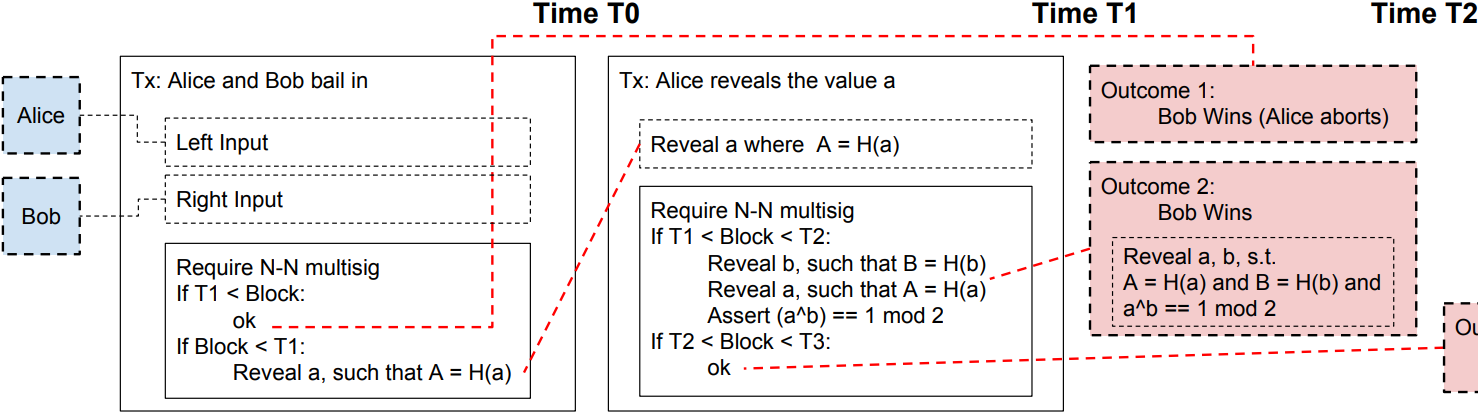
\includegraphics[width=\textwidth]{miller-bentov.png}
    \end{figure}
\end{frame}

%------------------------------------------------
\section{Scriptless Lottery}
\begin{frame}{Scriptless Lottery}
How do  we get our lottery to look like this?
\begin{figure}
    \centering
    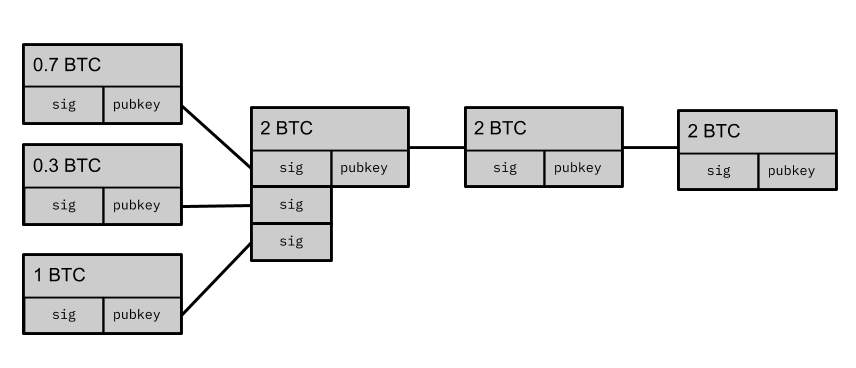
\includegraphics[width=\textwidth]{chain_view_2.png}
\end{figure}
\end{frame}

%------------------------------------------------

\begin{frame}{Oblivious transfer}
    \pause
    \begin{enumerate}
        \item  Manuel Blum to the rescue (again)! He made another discovery in 1981: you can generate a random outcome with oblivious transfer.
        \item  University of Berkeley technical report: \textit{Three applications of oblivious transfer: 1. Coin flipping by telephone, 2. How to exchange secrets, 3. How to send certified electronic mail}.
    \end{enumerate}

    \linebreak
    
    \pause
    \textbf{Rough Definition:}
    \begin{enumerate}
        \item Alice transmits one of $n$ message to Bob of Bob's choosing (But Alice doesn't learn which message).
        \item \textbf{receiver security} Sender doesn't know which message was sent
        \item \textbf{sender security} Receiver only gets one message
    \end{enumerate}
    
\end{frame}

%------------------------------------------------

\begin{frame}

\begin{figure}[!htb]
    \centering
    \[
\begin{array}{l c r}
Alice \hspace{4em} & & Bob \\
\hline \\
m_0,m_1 \getsdollar{} \{0,1\}^{k} &  &  b_2 \getsdollar{} \{0,1\}\\
&  & \\
 &  \rightleftarrows{} \textsf{OT}((b_2), (m_0,m_1)) \leftrightarrows{} & \text{learns $m_{b_2}$}  \\
& & \\
b_1 \getsdollar{} \{0,1\} &  b_1 & \\
 & \xlongrightarrow{\hspace{5em}} &\Rightarrow b_1 \oplus b_2 \\
& m' & \\
& \xlongleftarrow{\hspace{5em}} & \\
 b_2' \coloneqq \left\{ \begin{array}{l r}
         0  & m' = m_0 \\
         1 & m' = m_1  \\
         \bot & \text{otherwise} \\ \end{array} \right.
         & & \\
\Leftarrow b_1 \oplus b_2'  & & 
\end{array}
\]
\end{figure}

    
\end{frame}

%------------------------------------------------
%TODO: Put back "Alice broadcasts"

\begin{frame}
\begin{multicols}{2}
\begin{enumerate}
    \item<2-> Choose keys securely
    \item<3-> Sign the transaction scaffold
    \item<4-> Alice \textbf{obliviously signs} $\texttt{BobWin}$
    \item<5-> Sign and broadcast \texttt{Fund}
\end{enumerate}
\end{multicols}
    \begin{figure}
        \centering
        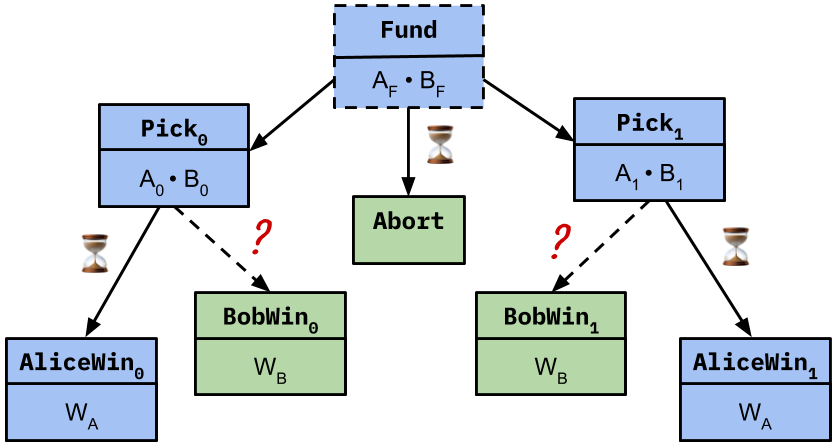
\includegraphics[width=\textwidth]{oblivious_signing_3.png}
    \end{figure}
\end{frame}

% \begin{frame}{Generating Keys fairly}
% Use hash commitment coin tossing! Choose keys randomly.

% \begin{enumerate}
%     \item $\mathbf{R}$ denotes $R_{\texttt{Abort}}, R_{\texttt{Choose}_0}, R_{\texttt{Choose}_1}, R_{\texttt{AliceWin}_0}, R_{\texttt{AliceWin}_1}, R_{\texttt{BobWin}_0}, R_{\texttt{BobWin}_1}$
%     \item Alice sends $c= H(r,A_F,A_0,A_1,\mathbf{R}_{\textsc{Alice}})$
%     \item Bob sends ($B_F,B_0,B_1, \mathbf{R}_{\textsc{Bob}}$)
%     \item Alice reveals $(r, A_F,A_0,A_1,\mathbf{R}_{\textsc{Alice}})$ and Bob checks against $c$
%     \item Both calculate the joint public keys and nonces as $A_F \cdot B_F$ etc 
% \end{enumerate}

% The above ensures neither party can adaptively choose their keys.
% \end{frame}

%------------------------------------------------
\begin{frame}{How to realise Oblivious Signing?}
    
    We want Bob to have a signature on $\texttt{BobWin}_0$ OR $\texttt{BobWin}_1$ but without Alice knowing which one.
    \pause
    \newline
    \newline
    \textbf{Approach}: Use adaptor signatures where Bob only knows the completion for one of them.
\end{frame}

%------------------------------------------------

\begin{frame}{Adaptor Signatures (Poelstra 2017)}
    Adaptor signatures enable the signer to create a simple access structure to a particular signature on a particular message.
    \\
    \begin{center}
    \begin{tabular}{|c|c|c|}
       \hline
       & Schnorr & Adaptor \\ \hline
       args & $sk, m$  &  $sk, m, Y = g^y$ \\ \hline
       $s = $& $r + H(g^r || pk || m)sk$ & $r + H(g^rY || pk || m)sk$  \\ \hline
       valid & $(s, g^{r})$ & $(s + y, g^{r}Y )$ \\ \hline
    \end{tabular}
    \end{center}
    \pause
    \textbf{Important feature}: The signer learns $y$ if they see the completed signature.
    
\end{frame}
%------------------------------------------------
\begin{frame}{Oblivious Signing}
    \textbf{Approach:} Alice to give Bob adaptor signatures where Bob only knows the completion for one of them.
    \pause
    \begin{itemize}
        \item<1-> A Pedersen commitment for $x$ is in the form $T = g^xh^c$.
        \item<2-> It's impossible to decommit to more than one value without knowing the DLOG$_g(h)$
        \item<3-> Fix $c \in \{0,1\}$, committer can only know discrete log of $T$ OR $Th^{-1}$
        \begin{itemize}
            \item $c = 0 \xlongrightarrow{} T = g^x$ (knows DLOG$(T))$
            \item $c = 1 \xlongrightarrow{} T = g^{x}h$ (knows DLOG$(Th^{-1})$)
        \end{itemize}
    \end{itemize}
\end{frame}

%------------------------------------------------

\begin{frame}{Oblivious Signing}


\begin{figure}[!htb]
    \centering
    \[
    \begin{array}{l c r}
        Alice(sk) & (m_0,m_1, h) & Bob(pk, c \in \{0,1\}) \\
        \hline \\
        & & y \getsdollar{} \mathbb{Z}_q\\
        & T = g^{y}h^{c} & \\
        & \xlongleftarrow{\hspace{5em}}  & \\ 
        (s_0,R_0) = \sigma(sk, m_0, T) & & \\
        (s_1,R_1) = \sigma(sk, m_1, T\inv{h}) & & \\
        & (s_0,R_0), (s_1,R_1) & \\
        & \xlongrightarrow{\hspace{5em}} & \\
        & & \textit{verify both} \\
        & & (s_c + y,  R_c \cdot g^{y}) \Rightarrow \\
    \end{array}
    \]
\end{figure}
\end{frame}

%------------------------------------------------

\begin{frame}{Secure?}

\begin{enumerate}
    \item<1-> \textbf{security for sender (Alice)}: If Bob can complete both adaptor signatures then he can solve $DLOG(h)$ (from the completion of both adaptor signatures we learn $DLOG$ of $T, Th^{-1}$).
    \item<2-> \textbf{security for receiver (Bob)}: It's information theoretically impossible for Alice to learn which choice Bob made (until he reveals it).
    \item<3-> Original protocol due to:
Tso R., Okamoto T., Okamoto E. (2008) 1-out-of-n Oblivious Signatures. In: Chen L., Mu Y., Susilo W. (eds) Information Security Practice and Experience. ISPEC 2008. Lecture Notes in Computer Science, vol 4991. Springer, Berlin, Heidelberg
    
\end{enumerate}
    
\end{frame}


\begin{frame}
Not so fast! Our transactions outputs are locked by joint public keys!
    \begin{figure}
        \centering
        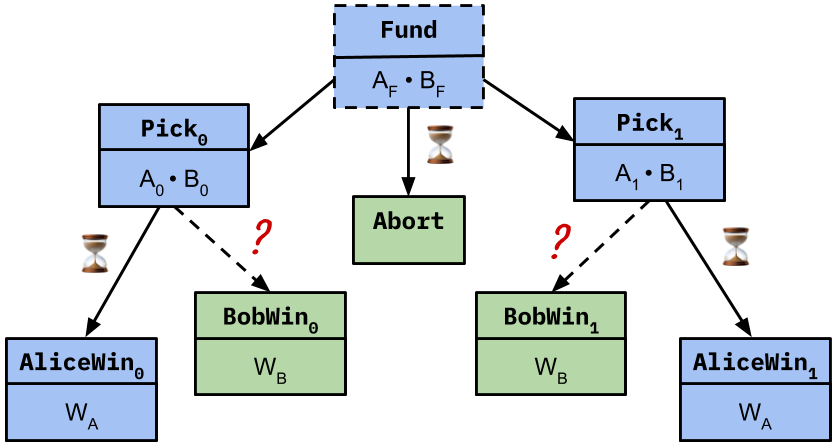
\includegraphics[width=\textwidth]{oblivious_signing_3.png}
    \end{figure}
\end{frame}


\begin{frame}{Two-party oblivious signing}
    One party knows which of two messages they are both signing but the other doesn't. Make a few changes:
    
    \begin{enumerate}
        \item They first choose joint nonces $R_{\texttt{BobWin}_0}, R_{\texttt{BobWin}_1}$ (we did this already).
        \item Along with $T$ Bob sends half adaptor signatures for $m_0$ ($\texttt{BobWin}_0$) and $m_1$ ($\texttt{BobWin}_1$) under $B_0$ and $B_1$
        \item Alice calculates the full adaptor signatures and sends them back to Bob
    \end{enumerate}
    
\end{frame}

\begin{frame}{Ok Done!}

    \begin{figure}
        \centering
        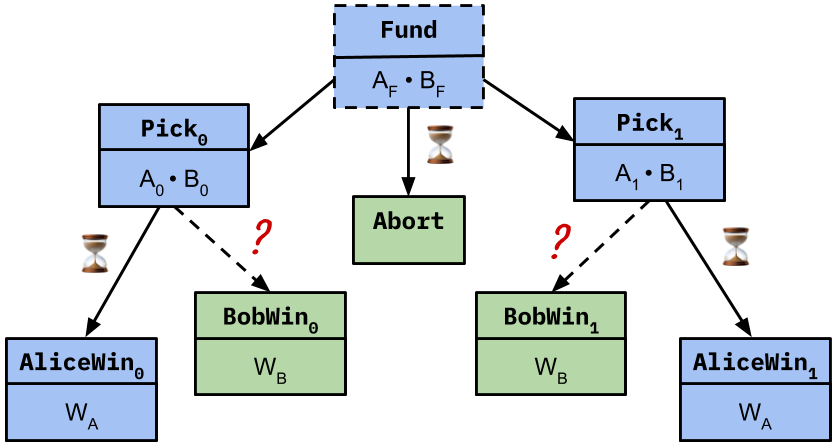
\includegraphics[width=\textwidth]{oblivious_signing_3.png}
    \end{figure}

\end{frame}


% \begin{frame}{Optimizing for cooperative parties}
%     Once the \texttt{Fund} transaction is confirmed:
%     \begin{enumerate}
%         \item Alice says: ``My choice is 1 so you won if you chose 0'' and sends the private key of $A_0$ (Alice will immediately lose if she plays $\texttt{Choose}_0$)
%         \item If Bob chose 1 he lost. He just sends his private key for $B_F$. Otherwise he chose 0 and won so he proves this to Alice by sending his completed signature on $\texttt{BobWin}_1$
%         \item If Bob has the signature, Alice now just sends him $A_F$
%         \item The winner now knows the private key for \texttt{Fund}'s output
%     \end{enumerate}
%     If either party aborts the off-chain protocol, just continue the on-chain protocol.
% \end{frame}

% \begin{frame}{Chain view of optimized protocol}
%     \begin{figure}
%         \centering
%         \includegraphics[width=\textwidth]{optimized_chain_view_1.png}
%     \end{figure}
% \end{frame}

\begin{frame}{Summary}
\textbf{Summary:}
\begin{itemize}
    \item<1-> Previous lottery protocols required sophisticated use of script.
    \item<2-> Using oblivious signing you can do a lottery without script that is more efficient on-chain.
    \item<3-> Oblivious signing with Schnorr signatures is efficient and secure (at least as it is used here).
\end{itemize}

\pause
\pause
\pause

\textbf{Unsubstantiated claims:}
\begin{itemize}
    \item You can do lotteries with different odds by doing $1/N$ oblivious signing rather than $1/2$.
    \item You can cooperatively complete the lottery in two on-chain transactions.
    \item You can execute cooperative protocol in a payment channel (and even do it "multi-hop" I think).
\end{itemize}

\end{frame}

% \begin{frame}{Channel}

% You can do this in a payment channel. You can could even do it ``multi-hop'' so that the player in the middle offsets their win or loss with a neighbor.

% \begin{figure}
%     \centering
%     \[
%      \begin{array}{c c c | c c c}
%      Bob          &                     &  Alice          &   Bob            &                     &  Alice \\
%      \textsf{P}_1 & \Longleftrightarrow & \textsf{Lloyd}  &   \textsf{Lloyd} & \Longleftrightarrow & \textsf{P}_2\\
%     \end{array}
%     \]
% \end{figure}



% \begin{enumerate}
%     \item Lloyd receives $T$ from $\textsf{P}_1$ and forwards it to $\textsf{P}_2$
%     \item When $\textsf{P}_2$ makes her choice, Lloyd makes the same choice with $\textsf{P}_1$.
%     \item If $\textsf{P}_1$ wins, then Lloyd is able to extract $\textsf{DLOG}_{g}(Th^{-c})$ from the completed signature and then win against $\textsf{P}_2$.
%     \item The timeouts have to longer between Lloyd and $\textsf{P}_2$
% \end{enumerate}
    
% \end{frame}

% \begin{frame}{What about Taproot?}
%     Taproot is a new proposal to secretly commit to a script in a normal looking public key.
%     \[ 
%         Q = P \cdot g^{H(P \Vert \texttt{script})}
%     \]
%     $P$ is the \textit{internal} public key and $Q$ is the \textit{external} public key.
%     \linebreak
%     \linebreak
%     \pause
%     \begin{enumerate}
%         \item Still have to reveal script in case of non-cooperation.
%         \item Even in the cooperative case, there is still \texttt{script} for the other party to leak later on.
%     \end{enumerate}
    
% \end{frame}


% \begin{frame}{Other potential applications of oblivious signing}

% \begin{enumerate}
%     \item<1-> Forcing cooperation for state update requests
%     \item<2-> ???
% \end{enumerate}

% \end{frame}

% \begin{frame}
% \frametitle{The Story of Satoshi Dice}
% \begin{itemize}
%     \item SatoshiDICE from 2012 to 2013 accounted for more than $50\%$ of Bitcoin transactions
%     \item It brought the blocksize limit into conciousness
% \end{itemize}
% \begin{figure}
%     \centering
%     \includegraphics[width=\textwidth]{satoshi_dice.png}
%     \caption{Caption}
%     \label{fig:my_label}
% \end{figure}
% \end{frame}



%-------------rand-----------------------------------

% \begin{frame}
% \frametitle{}
% \begin{columns}[c] % The "c" option specifies centered vertical alignment while the "t" option is used for top vertical alignment

% \column{.45\textwidth} % Left column and width
% \textbf{Heading}
% \begin{enumerate}
% \item Statement
% \item Explanation
% \item Example
% \end{enumerate}

% \column{.5\textwidth} % Right column and width
% Lorem ipsum dolor sit amet, consectetur adipiscing elit. Integer lectus nisl, ultricies in feugiat rutrum, porttitor sit amet augue. Aliquam ut tortor mauris. Sed volutpat ante purus, quis accumsan dolor.

% \end{columns}
% \end{frame}

% %------------------------------------------------
% \section{Second Section}
% %------------------------------------------------

% \begin{frame}
% \frametitle{Table}
% \begin{table}
% \begin{tabular}{l l l}
% \toprule
% \textbf{Treatments} & \textbf{Response 1} & \textbf{Response 2}\\
% \midrule
% Treatment 1 & 0.0003262 & 0.562 \\
% Treatment 2 & 0.0015681 & 0.910 \\
% Treatment 3 & 0.0009271 & 0.296 \\
% \bottomrule
% \end{tabular}
% \caption{Table caption}
% \end{table}
% \end{frame}

% %------------------------------------------------

% \begin{frame}
% \frametitle{Theorem}
% \begin{theorem}[Mass--energy equivalence]
% $E = mc^2$
% \end{theorem}
% \end{frame}

% %------------------------------------------------

% \begin{frame}[fragile] % Need to use the fragile option when verbatim is used in the slide
% \frametitle{Verbatim}
% \begin{example}[Theorem Slide Code]
% \begin{verbatim}
% \begin{frame}
% \frametitle{Theorem}
% \begin{theorem}[Mass--energy equivalence]
% $E = mc^2$
% \end{theorem}
% \end{frame}\end{verbatim}
% \end{example}
% \end{frame}

% %------------------------------------------------

% \begin{frame}
% \frametitle{Figure}
% Uncomment the code on this slide to include your own image from the same directory as the template .TeX file.
% %\begin{figure}
% %\includegraphics[width=0.8\linewidth]{test}
% %\end{figure}
% \end{frame}

% %------------------------------------------------

% \begin{frame}[fragile] % Need to use the fragile option when verbatim is used in the slide
% \frametitle{Citation}
% An example of the \verb|\cite| command to cite within the presentation:\\~

% This statement requires citation \cite{p1}.
% \end{frame}

% %------------------------------------------------

% \begin{frame}
% \frametitle{References}
% \footnotesize{
% \begin{thebibliography}{99} % Beamer does not support BibTeX so references must be inserted manually as below
% \bibitem[Smith, 2012]{p1} John Smith (2012)
% \newblock Title of the publication
% \newblock \emph{Journal Name} 12(3), 45 -- 678.
% \end{thebibliography}
% }
% \end{frame}

% %------------------------------------------------

\begin{frame}
\Huge{\centerline{The End}}
\end{frame}

%----------------------------------------------------------------------------------------

\end{document} 